\documentclass[12pt]{article}
\usepackage{amsmath}
\usepackage{graphicx}
\usepackage{caption}
\usepackage{subcaption}
 \usepackage[russian]{babel}
\usepackage{booktabs}
\usepackage{float}
\usepackage{minted}
\usepackage{verbatim}
\usepackage[utf8]{inputenc}
\usepackage{geometry}
\usepackage{multirow}
\usepackage{setspace}
\usepackage{parskip}
\usepackage[bottom]{footmisc}
\usepackage{tikz}
\usepackage[section]{placeins}

% This style is used to create block diagrams, you'll find it useful since many of your figures would be of that form, I'll try add more styles in the future :)
\usetikzlibrary{trees,positioning,fit,calc}
\tikzset{block/.style = {draw, fill=blue!20, rectangle,
                         minimum height=3em, minimum width=4em},
        input/.style = {coordinate},
        output/.style = {coordinate}
}

\usepackage[section]{minted}
\usepackage{xcolor}
\usemintedstyle{porland}

\usepackage{chngcntr}
\counterwithin{figure}{section}

\renewcommand{\arraystretch}{1.5}

\usepackage[hidelinks]{hyperref}
\hypersetup{
    linktoc=all
}

\renewcommand\listingscaption{Listing}
\renewcommand\listoflistingscaption{List of Listings}

\usepackage{scrhack}
\usepackage{tocbasic}
\setuptoc{lol}{levelup}

\usepackage{indentfirst}
\geometry{a4paper, margin=1in}

%----------EDIT COVER INFO HERE -----------------%

\def \LOGOPATH {assets/logo3.png}
\def \DEPARTEMENT {Министерство образования и науки Российской Федерации 
Федеральное государственное образовательное учреждение высшего образования
\\ «Национальный исследовательский университет «МЭИ» 
Институт ИВТ
Кафедра ПМИИ
}
\def \REPORTTITLE {Грамматический разбор методом рекурсивного спуска}
\def \STUDENTNAME {Желтиков Александр Алексеевич}
\def \STUDENTID {STUDNUM}


%------------------------------------------------%

\setlength{\parindent}{2em}
\setlength{\parskip}{0em}

\begin{document}

\pagenumbering{arabic}

\begin{titlepage}
    \vfill
    \begin{center}
        \includegraphics[width=0.7\textwidth]{\LOGOPATH} \\
        \hfill \\
        \Large{\DEPARTEMENT} \\
        \vfill
        \textbf{\LARGE{\REPORTTITLE}}
    \end{center}
    \vfill
    \begin{flushleft}
        \Large{\textbf{Отчет подгтовил:} \STUDENTNAME} \\
        \Large{\textbf{Дата:} \today}
    \end{flushleft}
    \vfill
\end{titlepage}

\clearpage

%------------------------------------------------%

\begin{center}
    \chapter{\textbf{\Large{Введение.}}}    
\end{center}
\\

\underline{\textit{\textbf{Задание.}}} Разработать алгоритм и реализовать программу для грамматического анализа методом рекурсивного спуска.
\\

\underline{\textit{\textbf{Часть 1.}}} Необходимо описать правила языка в форме БНФ. По данным правилам описать грамматику языка. Разработанную грамматику преобразовать к форме автоматной грамматики. Результаты показать преподавателю.
\\

\underline{\textit{\textbf{Часть 2.}}} По заданной грамматике построить ДКА, распознающий грамматику, и только её. Результаты показать преподавателю.
\\

\underline{\textit{\textbf{Часть 3.}}} Разработать алгоритм синтаксического анализа методом рекурсивного спуска
\\

\begin{center}
    \chapter{\textbf{\Large{Часть номер один.}}}    
\end{center}

\textbf{\underline{Program, var, begin, end, write, read, if, for, function, вызов функции}}
\\

\textbf{\underline{оператор присваивания,}}
\\

\textbf{\underline{арифметические операции + | - | * | /,}}
\\

\textbf{\underline{арифметические выражения}}
\\

\textbf{\underline{Типы данных: Integer, Boolean}}
\\

\begin{center}
    \chapter{\textbf{Опишем правила языка в форме БНФ для индивидуального варианта.}}
\end{center}

<program>::=<program title> ; <Block> .

<program title>::=program <name(identificatory)> 

<identificatory>::=<letters>  | <identificatory><letters> | <identificatory><numbers>

<letters>::= a | … | z  | A | … | Z

<numbers>::=0 | … | 9

<block>::=<description section><description section>

<description section>::=<variables section><procedures and function section>

<variables section>::= var<description var>  | <description var> <variables section>;

<procedures and function section>

\qquad\qquad\qquad\qquad\qquad\qquad\qquad               ::=    | <descript proc>;  |  | <description function>;| 

\qquad\qquad\qquad\qquad\qquad\qquad\qquad                         <procedures and function section> <description procedure>| 

\qquad\qquad\qquad\qquad\qquad\qquad\qquad                         <procedures and function section> <description function>            

<variables section>::= var<description var>  | <description var>   <variables section>;

<description var>::=<identificatory> ; <description var>  <identificatory>

<identificatory>::=<letters>  | <identificatory><letters> | <identificatory><numbers>

<compound operator>::=begin <list of operators> ; end. | begin end.

<list of operators>::=<operator>  | <operator> ; <list of operators>  <operator>;
<operator>

<write>::=write ( <list of expressions> )  | write()

<list of expressions>::=<text> | <expressions>

<text>::=<letters>  | <text>   <letters>

<expression>::=<Arithmetic expressions>

<read>::=read (<id>)  | read ()

<id>::=<identificatory> | <id> <identificatory>

<conditional operator> 

\qquad\qquad\qquad\qquad\qquad ::=if <logical expression> then <operator>|

\qquad\qquad\qquad\qquad\qquad if <logical expression> then <operator> else <operator>

<loop operator> 

\qquad::= for <loop parameter>:= <expression> to <expression> do <operator>  | 

\qquad      for <loop parameter>:= <expression> downto <expression> do <operator>

<loop parameter>::=<variable name>


<function>::=<function name> | <function name>(<list of actual parameters>)

\qquad    begin

 \qquad\qquad       <operators and in-block descriptions>

 \qquad   end;

<list of actual parameters>::=<actual parameters>  | <list of actual parameters>

\qquad\qquad\qquad\qquad\qquad\qquad\qquad\qquad\qquad<actual parameters>;

<actual parameters>::=<expression>  | <variable>  | <function name>  |  

\qquad\qquad\qquad\qquad\qquad\qquad\qquad\qquad\qquad<procedure name>


<function name>( [<list of formal parameters>] )  | 

<function name>();


<assignment operator>::= <variable>:=<expression> | <function name>:=<expression> 


<Addition operation>::=+  | - 

<Multiplication operation>::=*  | /  | mod  | div 


<Arithmetic expressions> 

\qquad  ::=<summand><Addition operation><summand> | 

      \qquad\qquad    <Arithmetic expressions> <summand>;


<type>::= <integer>  | <boolean> \\

\begin{center}
    \chapter{\textbf{Грамматика данного языка:}}    
\end{center}

G = (T, N, P, S)

\textit{\large{Множество терминальных символов T: }}

\{

Program,   var,   begin,   end,   write,   read,   if,   for,   function,   downto,   to,   do ,    const,   then,   else,   integer,   boolean,   a,  b,  c,  d,  e,  f,  g,  h,  i,  j,  k,  l,  m,  n,  o,  p,  q,  r,  s,  t,  u,  v,  w,  x,  y,  z,  A,  B,  C,  D,  E,  F,  G,  H,  I,  J,  K,  L,  M,  N,  O,  P,  Q,  R,  S,  T,  U,  V,  W,  X,  Y,  Z,  0,  1,  2,  3,  4,  5,  6,  7,  8,  9,  +,  -,  *,  div,  :=,  =,  <=, >=.<, >,  or,  and,  not,   “:” ,    “;” ,    “.” ,    “,  ” ,    “(“ ,    “)” 

\}

\textit{\large{Множество не терминальных символов N:}}

\{

<program title> , <identificatory>, <letters>, <numbers>, <block>,  <description section>, <variables section>, <procedures and function section>, <variables section>, <description var> <identificatory>, <compound operator> , <list of operators>, <write>,  <list of expressions>,<text>, <expression>, <read>, <id>, <conditional operator>, <loop operator>, <loop parameter>, <function>, <list of actual parameters>, <actual parameters>, <function name>,  <assignment operator>,  <Addition operation>, <Arithmetic expressions> <type>

\}

\textit{\large{Правила грамматики P:}}

<program>-><program title> ; <Block> .

<program title>->program <name(identificatory)> 

<identificatory>-><letters>  | <identificatory><letters> | <identificatory><numbers>

<letters>-> a | … | z  | A | … | Z

<numbers>->0 | … | 9

<block>-><description section><description section>

<description section>-><variables section><procedures and function section>

<variables section>-> var<description var>  | <description var> <variables section>;

<procedures and function section>

\qquad\qquad\qquad\qquad\qquad\qquad\qquad               ->    | <descript proc>;  |  | <description function>;| 

\qquad\qquad\qquad\qquad\qquad\qquad\qquad                         <procedures and function section> <description procedure>| 

\qquad\qquad\qquad\qquad\qquad\qquad\qquad                         <procedures and function section> <description function>            

<variables section>-> var<description var>  | <description var>   <variables section>;

<description var>-><identificatory> ; <description var>  <identificatory>

<identificatory>-><letters>  | <identificatory><letters> | <identificatory><numbers>

<compound operator>->begin <list of operators> ; end. | begin end.

<list of operators>-><operator>  | <operator> ; <list of operators>  <operator>;
<operator>

<write>->write ( <list of expressions> )  | write()

<list of expressions>-><text> | <expressions>

<text>-><letters>  | <text>   <letters>

<expression>-><Arithmetic expressions>

<read>->read (<id>)  | read ()

<id>-><identificatory> | <id> <identificatory>

<conditional operator> 

\qquad\qquad\qquad\qquad\qquad ->if <logical expression> then <operator>|

\qquad\qquad\qquad\qquad\qquad if <logical expression> then <operator> else <operator>

<loop operator> 

\qquad-> for <loop parameter>:= <expression> to <expression> do <operator>  | 

\qquad      for <loop parameter>:= <expression> downto <expression> do <operator>

<loop parameter>-><variable name>


<function>-><function name> | <function name>(<list of actual parameters>)

\qquad    begin

 \qquad\qquad       <operators and in-block descriptions>

 \qquad   end;

<list of actual parameters>-><actual parameters>  | <list of actual parameters>

\qquad\qquad\qquad\qquad\qquad\qquad\qquad\qquad\qquad<actual parameters>;

<actual parameters>-><expression>  | <variable>  | <function name>  |  

\qquad\qquad\qquad\qquad\qquad\qquad\qquad\qquad\qquad<procedure name>


<function name>( [<list of formal parameters>] )  | 

<function name>();


<assignment operator>-> <variable>:=<expression> | <function name>:=<expression> 


<Addition operation>->+  | - 

<Multiplication operation>->*  | /  | mod  | div 


<Arithmetic expressions> 

\qquad  -><summand><Addition operation><summand> | 

      \qquad\qquad    <Arithmetic expressions> <summand>;


<type>-> <integer>  | <boolean> \\

\textit{\large{Аксиома S:}}  <program>  \\


\begin{center}
    \chapter{\textbf{\Large{Часть номер два.}}}    
\end{center} \\
\centering{ДКА}
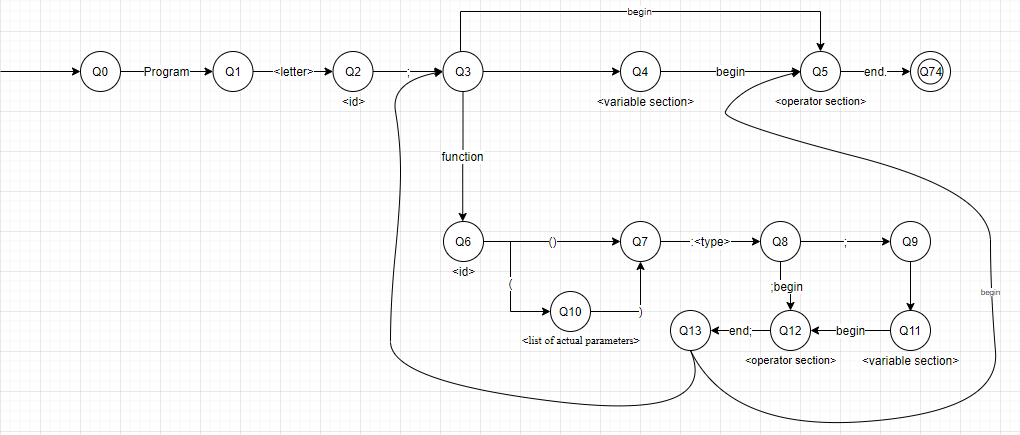
\includegraphics[width=1\textwidth]{assets/ДКА.png}

\centering{Оператор for}
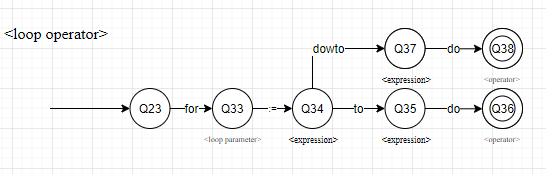
\includegraphics[width=1\textwidth]{assets/Оператор for.png}

\centering{Оператор if}
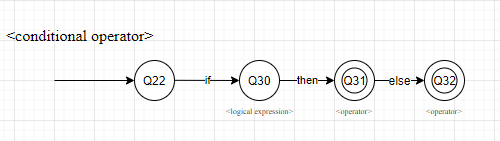
\includegraphics[width=1\textwidth]{assets/Оператор if.png}

\centering{Секция Var}
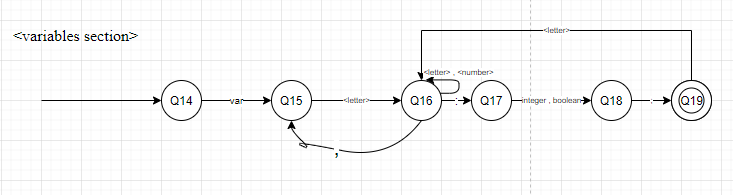
\includegraphics[width=1\textwidth]{assets/Секция Var.png}

\centering{Секция операторов}
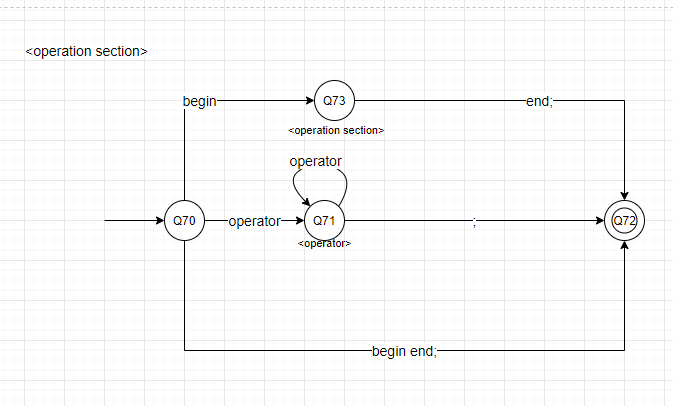
\includegraphics[width=1\textwidth]{assets/Секция Операторов.png}

\centering{Оператор записи и чтения}
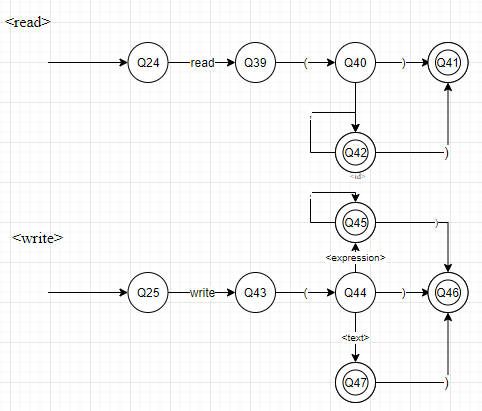
\includegraphics[width=1\textwidth]{assets/Оператор Записи и Чтения.png}

\centering{Оператор присваивания}
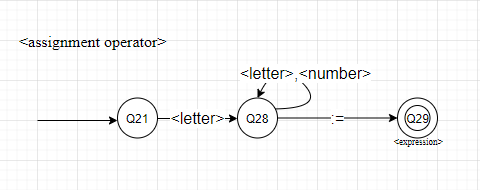
\includegraphics[width=1\textwidth]{assets/Оператор Присваивания.png}

\centering{Сравнения и Логические функции}
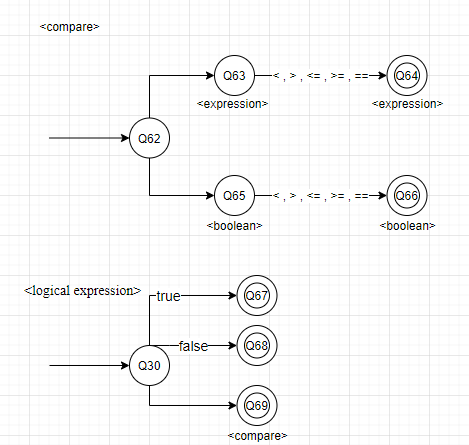
\includegraphics[width=1\textwidth]{assets/Сравнение и Логика.png}

\centering{Операторы}
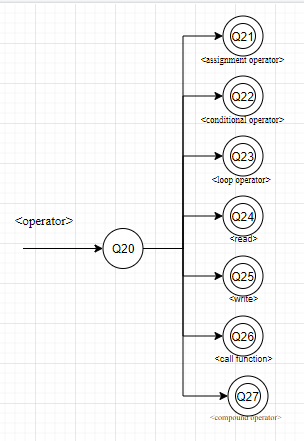
\includegraphics[width=0.8\textwidth]{assets/Операторы.png}

\centering{Обозначения переменных}
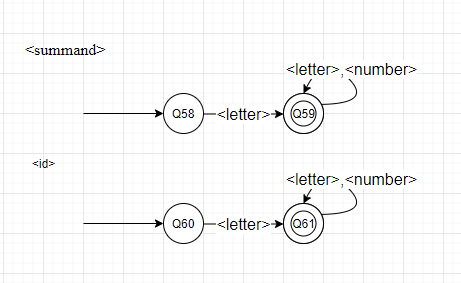
\includegraphics[width=1\textwidth]{assets/Обозначения переменных.png}

\centering{Вызов функции}
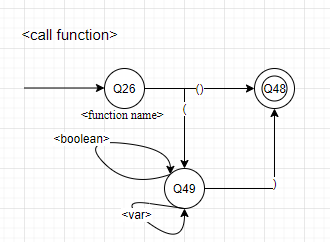
\includegraphics[width=1\textwidth]{assets/Вызов Функции.png}

\centering{Константы и выражения}
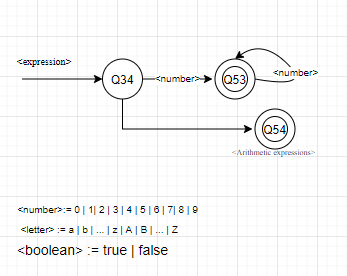
\includegraphics[width=0.7\textwidth]{assets/В конце.png}

\begin{center}
    \chapter{\textbf{\Large{Часть номер три.}}}    
\end{center}

\begin{flushleft}
Данный алгоритм имеет скорость O(n), тоесть линейную, где n - количество слов в исходной строке (или в исходном коде языка Паскаль). Работает алгоритм достаточно просто, мы токинезируем (разбиваем на ключевые слова) наш код и идем слева на право (методом рекурсивного спуска). При достижении определенных токенов, вызываются определенные функции. 
\end{flushleft}

\centering\textbf{Тестирование программы:}

\hline
Тест номер 1 -- Ожидаемый результат:\\
\begin{verbatim}
program abc;
var x,y,m,n:integer;
function MN(a,b:integer):integer;
   var max:integer;
begin
   if -2*a+b > b+a then if max = -a then a:= f else max := b else max := a;
   MaxNumber:=max;
end;
begin
   for i := 1 to 10 do
   i := 1+2*3;
   count:=MN(a,b);
   write(input x,y);
   read(x,y);
   write(m,n);
end.

#########################################################################

Начинаем проверку языка на корректность
Данный язык соответсвует языку паскаль!

\end{verbatim}
\hline


Тест номер 2 -- Ожидаемый результат:\\
\begin{verbatim}
program abc;
begin
end.

#########################################################################

Начинаем проверку языка на корректность
Данный язык соответсвует языку паскаль!

\end{verbatim}

\hline
Тест номер 3 -- Ожидаемый результат:\\
\begin{verbatim}
program abc
var x,y,m,n integer;
function MN(a,b:integer):integer;
   var max:integer;
begin
   if a+b > b ++ a then then max := a else max := b;
   MaxNumber:=max;
end;
begin
   for i := 1 to 10 do
   i := 1+2*3;
   write(input x,y);
   read(x,y);
   write(m,n);
end.



#########################################################################

Начинаем проверку языка на корректность
Ошибка находится в , Line ---> 1

\end{verbatim}
\hline

Тест номер 4 -- Ожидаемый результат:\\
\begin{verbatim}

program abc;
var x,y,m,n integer;
function MN(a,b:integer):integer;
   var max:integer;
begin
   if a+b > b ++ a then then max := a else max := b;
   MaxNumber:=max;
end;
begin
   for i := 1 to 10 do
   i := 1+2*3;
   write(input x,y);
   read(x,y);
   write(m,n);
end.


#########################################################################

Начинаем проверку языка на корректность
Ошибка находится в , Line ---> 2

\end{verbatim}
\hline

Тест номер 5 -- Ожидаемый результат:\\
\begin{verbatim}

program abc;
var x,y,m,n integer;
function MN(a,b:integer):integer;
   var max:integer;
begin
   if a+b > b+a then then max := a else max := b;
   MaxNumber:=max;
end;
begin
   for i := 1 to 10 do
   i := 1+2*3;
   write(input x,y);
   read(x,y);
   write(m,n);
end.


#########################################################################

Начинаем проверку языка на корректность
Ошибка находится в , Line ---> 6
\end{verbatim}
\hline

\textbf{Код программы:}

\begin{minted}[fontsize=\footnotesize]{c++}

#include <iostream>
#include <string>
#include <fstream>
#include <vector>

using namespace std;

int beginCount = 0; // Счётчик Begin-End
int countError = 0; // Счётчик ошибок
int countLine = 1; // Счётчик строк
bool flag = true;
int i = 0;
int check = 0;
vector<string> ourPascalLine;

void id(const string& s);
void ProgramBegin(const string& s);
void next(const string& s);
void Operator(const string& s);
void letter(const string& s);
void letterCheck(const string& s);
void conditionalOper(const string& s);
void createFunc(const string& s);
void nums(const string& s);
void loopoperator(const string& s);
void RWout(const string& s);

// Данная функция считывает все строки из файла 
//и заполняет одну единую строку для удобства.
//------------------------------------------------------------------------------------------
string ReadPascal(){
    ifstream file("/Users/pika4picha/Desktop/LabPart3/example1.txt");

    string x, line;

    if (file.is_open()){
        while(getline(file, x)){
            line += x + " ";
        }
        file.close();
    }
    else return "Can't file in our directory!";
    return line;
}
//------------------------------------------------------------------------------------------

//Данная функция переводит строку в вектор, тоесть полностью её разделяет.
//------------------------------------------------------------------------------------------
vector<string> splitLine(const string& line){
    vector<string> s;
    string foo;
    for(char ch : line){
        if(ch == ' '){
            if (foo != "") s.push_back(foo);
            foo = "";
            }
            else if(ch == ';')
            {
                if (foo != "") s.push_back(foo);
                foo = "";
                s.emplace_back(";");
            }
                else if(ch == ':')
                 {
                    if (foo != "") s.push_back(foo);
                    foo = ":";
                 }
                else if(ch == '(')
                {
                    if (foo != "") s.push_back(foo);
                    s.emplace_back("(");
                    foo = "";
                }
                else if(ch == ')')
                {
                    if (foo != "") s.push_back(foo);
                    s.emplace_back(")");
                    foo = "";
                }
                else if(foo == ":="){
                    s.push_back(foo);
                    foo = ch;
                }
                else foo += ch;
    }
    return s;
}
//------------------------------------------------------------------------------------------

// Функуия для запуска программы.
void ProgramBegin(const string& s){
    id(s);
}

// Функция проверяет совпадения Чисел и знаков.
void nums(const string& s){
    for(auto x : s){
        if(!((x >= 'a' && x <= 'z') || (x >= 'A' && x <= 'Z') || 
        (x >= '0' && x <= '9')
        || x == '+' || x == '-' || x == '/' || x == '*')) countError++;
    }
    if(countError > 0){
        cout << "Ошибка при обозначении программы, начинается 
        не с букв , Line " << countLine << "\n";
    }
    i++;
    next(ourPascalLine[i]);
}

// Проверяет названия переменных
void id(const string& s){
    if((s[0] >= 'a' && s[0] <= 'z') || (s[0] >= 'A' && s[0] <= 'Z')){
        for(auto x : s){
            if(!((x >= 'a' && x <= 'z') || (x >= 'A' && x <= 'Z')
            || (x >= '0' && x <= '9') )) countError++;
        }
    } else {
        countError++;
        cout << "Ошибка при обозначении программы, начинается
        не с букв , Line " << countLine << "\n";
    }
    i++;
    next(ourPascalLine[i]);
}

void letter(const string& s){
    if (s != "function"){
    if((s[0] >= 'a' && s[0] <= 'z') || (s[0] >= 'A' && s[0] <= 'Z') || s[0] == '-'){
        for(auto x : s){
            if(!((x >= 97 && x <= 122) || (x >= 65 && x <= 90) || 
            (x >= 48 && x <= 57) || x == ',' ||
                     x == '+' || x == '-' || x == '/' || x == '*')) countError++;
        }
    } else {
        countError++;
        cout << "Ошибка находится в , Line ---> " << countLine << "\n";
    }
    i++;
    next(ourPascalLine[i]);}
    else next(ourPascalLine[i]);
}

void letterCheck(const string& s){
    if (s == ";") {
        i++;
        countLine++;
        letterCheck(ourPascalLine[i]);
    }else if (s == "begin"){
        i++;
        countLine++;
        beginCount++;
        Operator(ourPascalLine[i]);
    } else {
        letter(ourPascalLine[i]);
    }
}

// Что-то на подобии функции перехода, она помогает нам идти дальше по коду Паскаля.
void next(const string& s){
    if (s == ";"){
        i++;
        countLine++;
        if (beginCount == 0) next(ourPascalLine[i]);
        else Operator(ourPascalLine[i]);
    } else if (s == "begin"){
        i++;
        countLine++;
        beginCount++;
        Operator(ourPascalLine[i]);
    } else if (s == "var"){
        i++;
        letter(ourPascalLine[i]);
    } else if (s == ":integer" || s == ":boolean") {
        if(check == 2) {i++; createFunc(ourPascalLine[i]);}
        else {
            i++;
            letterCheck(ourPascalLine[i]);
        }
    } else if (s == "=" || s == "<=" || s == ">=" || s == "<" || s == ">") {
        i++;
        check = 1;
        conditionalOper(ourPascalLine[i]);
    } else if (s == "function") {
        i++;
        check = 2;
        letter(ourPascalLine[i]);
    } else if (s == "(" && check == 2) {
        i++;
        createFunc(ourPascalLine[i]);
    }
        else if (s == ":=") {
            i++;
            Operator(ourPascalLine[i]);
    } else if (check == 1) {
        check = 0;
        conditionalOper(ourPascalLine[i]);
    } else if (s == "(") {
        i++;
        letter(ourPascalLine[i]);
    } else if (s == ")") {
        i++;
        next(ourPascalLine[i]);
    }
        else if (s == "+" ||
                   s == "-" || s == "/" || s == "*"){i++; Operator(ourPascalLine[i]);}
        else if (s == "to" || s == "downto") {i++; loopoperator(ourPascalLine[i]);}
        else if (s == "do") {i++; countLine++; Operator(ourPascalLine[i]);}
        else if (s == "else"){i++; Operator(ourPascalLine[i]);}
        else if (check == 4) {
        RWout(ourPascalLine[i]);
    }
    else if (countError == 0)cout << "Ошибка находится
    в , Line ---> " << countLine << "\n";
}

void createFunc(const string& s){
    if (s == ")") {i++; next(ourPascalLine[i]);}
    else if (ourPascalLine[i-1] == "(") letter(s);
    else {check = 0; next(s);}
}

void conditionalOper(const string& s){
    if(s == "then"){i++; countLine++; Operator(ourPascalLine[i]);}
    else {letter(ourPascalLine[i]);};
}

void loopoperator(const string& s){
    if (s[0] >= 48 && s[0] <= 57) {nums(s);}
}

void RWout(const string& s){
    if (s == "(") {i++ ; check = 4; RWout(ourPascalLine[i]);}
    else if (s == ")") {i++; check = 0 ; next(ourPascalLine[i]);}
    else {letter(ourPascalLine[i]);}
}

void Operator(const string& s){
    if (s == "if"){i++; conditionalOper(ourPascalLine[i]);}
    else if (s == "end"){i++;beginCount--; next(ourPascalLine[i]);}
    else if (s == "read" || s == "write") {i++ ; RWout(ourPascalLine[i]);}
    else if (s == ";"){i++; countLine++ ;next(ourPascalLine[i]); }
    else if (s == "for") {i++; Operator(ourPascalLine[i]);}
    else if (s == "begin") {i++; countLine++; beginCount++; 
        Operator(ourPascalLine[i]);}
    else if (s == "end." && countError == 0)
        cout << "Данный язык соответсвует языку паскаль!"<< "\n";
    else if ((s[0] >= 97 && s[0] <= 122) || (s[0] >= 65 && s[0] <= 90)) {letter(s);}
    else if ((s[0] >= '0' && s[0] <= '9') || s[0] == '+' || s[0] == '-' 
    || s[0] == '/' || s[0] == '*') {nums(s);}
    else next(ourPascalLine[i]);
}
int main() {

    ourPascalLine = splitLine(ReadPascal()); // Здесь происходит некая токинезация.
    // Наш вектор с языком паскаль с помощью него мы проверим правильность языка

    cout << "Начинаем проверку языка на корректность\n";

//    for(const auto& x : ourPascalLine)   /*   Можно использовать для вывода токенов.
//        cout << x << "\n";                */ 

    if (ourPascalLine[i] == "program"){
        ++i;
        ProgramBegin(ourPascalLine[i]);
    }
    if (countError != 0) cout << "К сожалению наш код не 
    будет распознаваться языком Паскаль...";
    return 0;
}

\end{minted}

\end{document}

